\documentclass[reprint,aip,apl,floatfix,linenumbers,superscriptaddress]{revtex4-1}
\usepackage{graphicx}
\usepackage[product-units = power]{siunitx}
\usepackage[version=3]{mhchem}
\usepackage[utf8]{inputenc}
\usepackage{natbib}
%\usepackage{stackengine}

\DeclareSIUnit\BohrMagneton{$\mu_B$}
\DeclareSIUnit\formulaunit{f.u.}
\DeclareSIUnit\atomicunit{a.u.}
\DeclareSIUnit\arbunit{arb.unit}
\DeclareSIUnit\torr{Torr}

\begin{document}

%title, authors, affiliations
\title{Transport properties of cubic zero-moment ferromagnetic \ce{Mn2Ru$_x$Ga
} thin films}
\author{Naganivetha Thiyagarajah}
\author{Yong-Chang Lau}
\author{Karsten Rode}
\author{Davide Betto}
\author{Kiril Borisov}
\author{M. Venkatesan}
\author{J. M. D. Coey}
\author{Plamen Stamenov}
\affiliation{CRANN, AMBER and School of Physics, Trinity College Dublin, 
Dublin 2, Ireland}

\date{\today}

%abstract needs to be written
\begin{abstract}
The spin-dependent transport properties of cubic \ce{Mn2Ru$_x$Ga} thin-films 
are studied as a function of the the Ru concentration, $x$ and the substrate 
induced strain. We find that at Ru concentration $x\approx\num{0.7}$, which 
shows practically zero magnetization, the spontaneous Hall effect at room 
temperature reverses sign and the spontaneous Hall angle is maximized. In 
addition, a small tetragonal distortion, $c/a\sim\num{2}\%$, allows us to 
tune the compensation of the two Mn sub-lattices to a preferred temperature 
at, above or below room temperature. Having two handles on the zero moment 
half magnetic properties of \ce{Mn2Ru$_x$Ga} opens up the possibilities for 
using this new class of material in various spintronic devices. We also 
present the initial work on magnetoresistive devices based on pseudo-spin-
valves with \ce{Mn2Ru$_x$Ga} electrodes.

\end{abstract}
\maketitle

%Introduction 
\section{Introduction}
\label{sec:intro}

Cubic ferromagnetic Heusler compounds are a family of magnetic materials that 
often exhibit higher spin polarization at the Fermi level than binary 
ferromagnetic $3d$ alloys\cite{Graf2013}. Some of the materials are half-
metals with a gap in the spin-polarized density of states for one spin band 
which should make them ideal candidates for spin-valves or MTJs\cite{PhysRevB.
28.1745,Wang2009,Takahashi2011,Tsunegi2008}.  Since the prediction by van 
Leuken and de Groot in $1995$, of a half-metallic material with two in-
equivalent magnetic sub-lattices whose moments cancel out \cite{PhysRevLett.50
.2024}, researchers have worked on fabricating such a material. While 
electronic structure calculations predicted several such compounds\cite{
Wurmehl2006, Hu2012, Galanakis2006}, fabrication of such materials had failed
\cite{Hu2012,PhysRevB.79.100406}. In $2014$, Kurt \textit{et. al.} reported 
the growth of thin films of \ce{Mn2Ru$_x$Ga} (\ce{MRG}), which was identified 
as a zero-moment ferrimagnet with high spin polarization and showed evidence 
of half-metallicity\cite{KurtPRL2014}. 

Here we report on the temperature, composition and thickness dependent 
transport properties of \ce{MRG}, which are at or near compensation point ($0.
6<x<1.1$). Addition of Ru to the cubic \ce{Mn2Ga} structure provides both 
states (\num{12}) and electrons (\num{8}). Based on the on the empirical 
Slater-Pauling rules, should result in perfect compensation for \ce{Mn2Ru$_{0.
5}$Ga}. However the addition of Ru is likely to change both the shape and 
position of the Mn bands leading to a more complex behaviour of the magnetic 
and spin-dependent transport properties. In addition the tetragonal 
distortion ($c/a$) can also affect the band structure, hence we also look at 
strain as a possible control parameter in engineering the \ce{MRG} fully 
compensated half metallic system.


%experiment 
\section{Experimental techniques}
\label{sec:exp_tech}

\ce{MRG} films of thickness \SIrange{4}{70}{\nano\metre} were grown on \ce{MgO
} (001) substrates by dc-magnetron sputtering at \SI{250}{\celsius} substrate 
temperature and base pressure \SI{2e-8}{\torr} in a Shamrock deposition 
system. The films were co-sputtered from a Mn2Ga target and Ru target, and 
the Ru composition was controlled by keeping the \ce{Mn2Ga} sputtering power 
fixed while varying that of Ru. The MRG films were capped with a  $\sim \SI{2
}{\nano\metre}$ \ce{Al2O3} layer to prevent oxidation.  The crystal structure 
and lattice parameters were determined by $2\theta-\theta$ and reciprocal 
space map (RSM) scans using a BRUKER D8 diffractometer. In order to determine 
the \ce{Ru} concentration $x$, we deposited four samples with varying \ce{Mn2
Ga} target power along with a \ce{Ru} film. The density and thickness of the 
samples were then measured using x-ray reflectivity. Based on the measured 
density and lattice parameters of these 5 control samples, we establish a 
relation between the x-ray density and the \ce{Ru} concentration $x$ against 
which all the samples are calibrated. Magnetization measurements were made 
using a Quantum Design superconducting quantum interference device (SQUID) 
magnetometer. The transport measurements were conducted on unpatterned \ce{MRG
} films in a physical properties measurement system (PPMS) for temperatures 
from \SIrange{10}{400}{\kelvin}. The maximum applied magnetic fields, $\mu_0H$
, for the two systems were \SI{5}{\tesla} and \SI{14}{\tesla} respectively. A 
summary of sample properties is provided in Table \ref{tab:samples}. We also 
incorporated the \ce{MRG} as the hard layer into a pseudo-spin-valve with the 
structure, \ce{MgO}/ \ce{MRG}(15)/\ce{Cu}(2.8)/[\ce{Co}(0.2)/\ce{Pd}(0.6)]$_6$
/\ce{Ta}(\SI{3}{\nano\metre}) in order to investigate the spin dependent 
transport. The \ce{MRG} layer was grown at \SI{250}{\celsius}, then cooled 
down to room temperature, and was subsequently transferred to a different 
deposition chamber for the \ce{Cu}/[\ce{Co}/\ce{Pd}] multilayer deposition. 
Atomic force microscopy measurements of the \ce{MRG} film showed a roughness 
of $\sim \SI{0.2}{\nano\metre}$, free of pinholes. 

%table with properties
\begingroup
\squeezetable
\begin{table}
  \caption{Summary of sample properties. The temperature at which full compensation occurs, $T_{comp}$ was defined by the temperature where $\partial \rho_{xy}/\partial T$ reaches its maximum.}
  \begin{ruledtabular}
  \begin{tabular}{c c c c c }
    \ce{Ru} $x$ & $t$ &  $c/a-1$ & $M_s$ & $T_{comp}$ \\ 
		 & \SI{}{\nano\metre} & \SI{}{\percent} & \SI{}{\BohrMagneton}  & \SI{}{\kelvin} \\
     \hline
     \num{0.62} & \num{70} & \num{2.07} & \num{-0.09} & \numrange[range-phrase = --]{100}{200} \\ 

%NT059
     \num{0.69} & \num{70} & \num{1.76} & \num{0.03} & \numrange[range-phrase = --]{200}{300} \\ %NT058
     \num{0.73} & \num{70} & \num{1.83} & \num{0.07} & \numrange[range-phrase = --]{300}{360} \\ %NT063
		 \num{0.77} & \num{70} & \num{1.92} & \num{0.09} & \num{> 360} \\ %NT055
		 \num{1.09} & \num{70} & \num{1.82} & \num{0.07} & \num{> 360} \\ %NT046
     \num{1.12} & \num{70} & \num{1.84} & \num{0.07} & \num{387} \\ %NT072 
		 \num{1.01} & \num{34} & \num{1.92} & - & \num{335} \\ %NT073
		 \num{0.98} & \num{16} & \num{2.24} & - & \num{280} \\ %NT074
     \num{1.09} & \num{8} & \num{2.90} & - & \num{214} \\ %NT075
		 \num{1.07} & \num{4} & \num{3.60} & - & \num{< 10} \\ %NT076	 
  \end{tabular}
  \end{ruledtabular}
  \label{tab:samples}
\end{table}
\endgroup

%results section needs to be expanded - more discussion
\section{Results and Discussion}
\label{sec:results_discussion}

%fig 0 - XRD - some tweaking
\begin{figure}
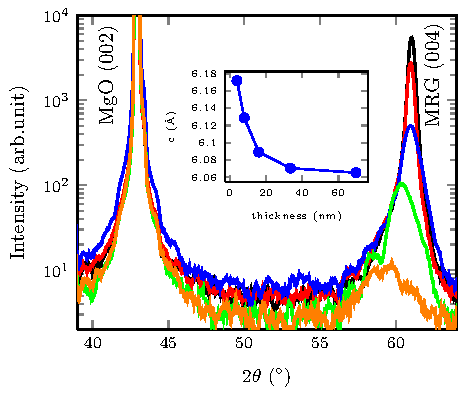
\includegraphics[width=1.0\columnwidth]{Transport-Fig0.pdf}
\caption{XRD of thin films of \ce{Mn2Ru$_x$Ga} of thickness from \SIrange{70}{
4}{\nano\metre} grown on \ce{MgO} substrates. Inset shows the dependence of 
the out-of-plane lattice parameter (c) on the thickness of the film, 
indicating that the substrate induced strain is increasingly relaxed as the 
thickness increases.}
\label{fig:xrd}
\end{figure}

The crystal structure of the cubic \ce{MRG} films with different thickness 
and compositions were probed using $2\theta-\theta$ x-ray diffraction (XRD) 
as shown in Fig. \ref{fig:xrd}. The out-of-plane lattice parameter, $c$, is 
between \SI{0.598}{\nano\metre} and \SI{0.618}{\nano\metre}, depending on the 
\ce{Ru} concentration and film thickness (insert of Fig. \ref{fig:xrd}). The 
in-plane lattice parameter, $a$, determined from reciprocal space maps was 
found to be \SI{0.596}{\nano\metre} for all samples, which is precisely 
matched to that of the \ce{MgO} substrate ($\sqrt{2} a_0\left(\ce{MgO} \right)
 = \SI{0.5956}{\nano\metre}$). This confirms the cubic nature of the \ce{MRG} 
films with a slight tetragonal out-of-plane distortion ($c/a-1$ between \num{1
.8}\% and \num{3.6}\%).

%fig 1 - SQUID ok - is it needed? 
\begin{figure}
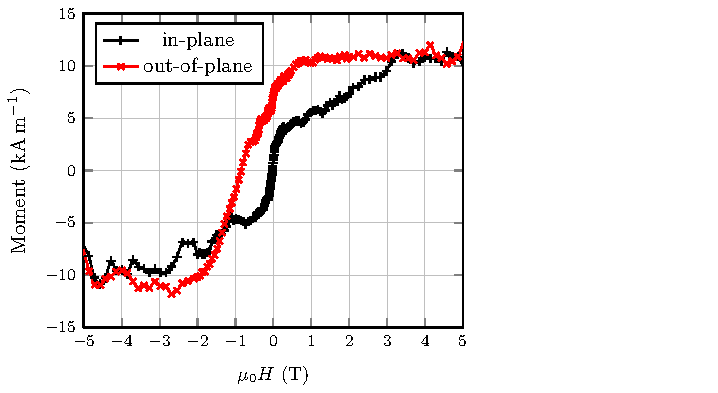
\includegraphics[width=1.5\columnwidth]{Transport-Fig1.pdf}
\caption{In-plane and out-of-plane magnetization loops of \ce{Mn2Ru$_x$Ga} 
sample of thickness \SI{70}{\nano\metre}, measured in a SQUID magnetometer at 
\SI{300}{\kelvin}.}
\label{fig:squid}
\end{figure}

%fig 2 - ehe curves of Ru_conc and temp dependence? 
\begin{figure}
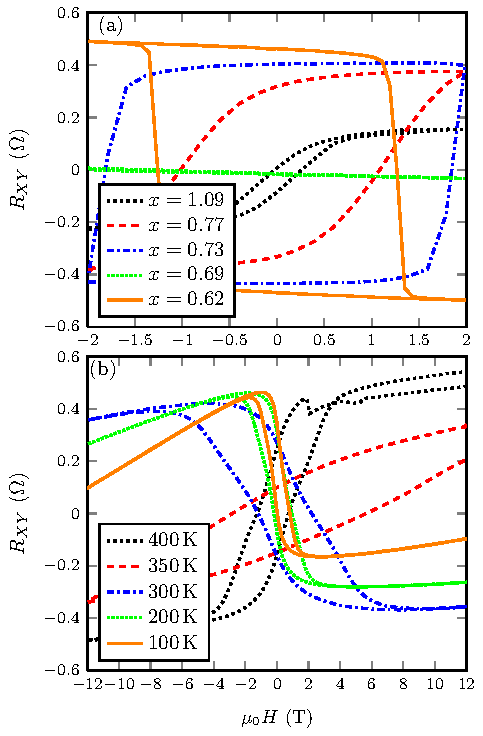
\includegraphics[width=1.0\columnwidth]{Transport-Fig2.pdf}
\caption{SHE loops measured of \ce{Mn2Ru$_x$Ga} for (a) various Ru 
compositions ($0.6<x<1.1$) and (b) temperatures between \SI{10}{\kelvin} and 
\SI{400}{\kelvin}, which illustrates the change of sign of the spontaneous 
hall coefficient between $x=0.62$ and $x=0.73$ and \SI{300}{\kelvin} and \SI{
350}{\kelvin} respectively.}
\label{fig:she}
\end{figure}

%figure3 - Ru conc ms and ehe params
\begin{figure}
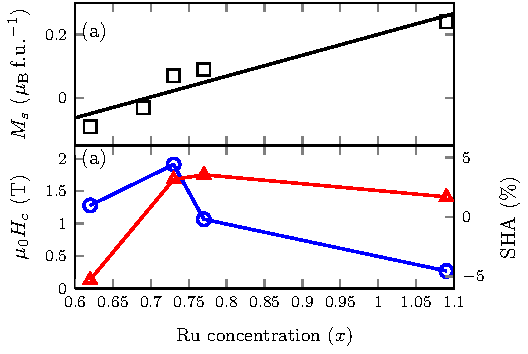
\includegraphics[width=1.0\columnwidth]{Transport-Fig3.pdf}
\caption{(a) Extracted magnetization at \SI{300}{\kelvin} (in \SI{}{
\BohrMagneton\per\formulaunit}), for samples of thickness \SI{70}{\nano\metre}
 with different \ce{Ru} composition ($0.6<x<1.1$). The change of sign of the 
magnetization was established by SHE sign reversal at compensation. (b) 
Coercive field  and spontaneous Hall angle as a function of \ce{Ru} 
composition, extracted from SHE measurements carried out at \SI{300}{\kelvin}
, for the same \ce{MRG} samples as in (a).}
\label{fig:ru_conc}
\end{figure}

Fig. \ref{fig:squid} shows the magnetization measurement at \SI{300}{\kelvin} 
of a typical \ce{MRG} film of \SI{70}{\nano\metre} near compensation of the 
magnetic sub-lattices. Clear out-of-plane anisotropy with a large coercivity 
of \SI{1.2}{\tesla} is evident.  A small soft in-plane component is also 
clearly visible. As the \ce{Ru} concentration is reduced from $x=\num{1.09}$, 
the magnetization reduces, until it falls practically to zero (\SI{12}{
\kilo\ampere\per\metre} or \SI{0.07}{\BohrMagneton\per\formulaunit}) at $x=
\num{0.68}$ as shown in Fig. \ref{fig:ru_conc}(a). We can attribute this to 
the almost perfect compensation of the two \ce{Mn} sub-lattices at room 
temperature. On further reduction of Ru the magnetization again increases. We 
denote this as a negative magnetization, coincident with the reversal in sign 
in the room temperature spontaneous Hall effect (SHE) measurements as shown 
in Fig. \ref{fig:she}(a). From the SHE measurements with varying Ru content, 
we extracted the coercivity, $\mu_0H_c$, and spontaneous Hall angle (SHA) (
defined as $\rho_H$/$\rho$) (Fig. \ref{fig:ru_conc}(b)). As the magnetization 
approaches zero the coercivity clearly diverges (the sample closest to 
compensation at room temperature could not be saturated at an applied field 
of \SI{5}{\tesla}). The recorded SHA for samples near compensation ($\sim \num
{5}\%$) are about a magnitude larger than those reported for other 3d 
ferromagnets at room temperature (\numrange{0.2}{0.3}\%)\cite{dorleijn1976} 
and comparable to SHA recorded for amorphous rare earth transition metal 
alloys\cite{Kim2001}. A high SHA is indicative of much lower carrier 
concentrations and a high spin polarization.

%fig 4 on strain/thickness goes here
\begin{figure}
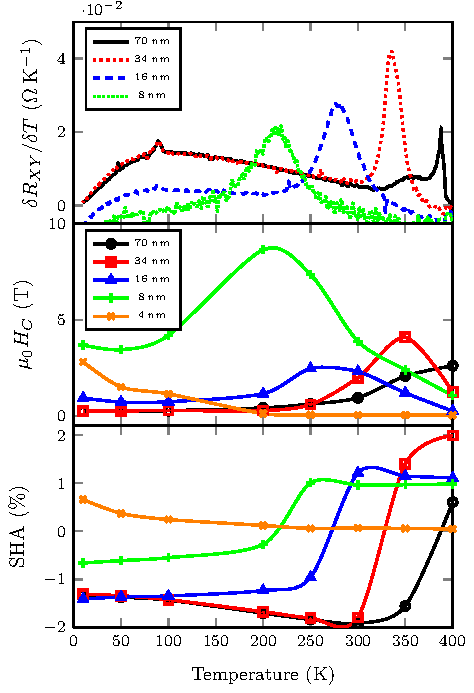
\includegraphics[width=1.0\columnwidth]{Transport-Fig4.pdf}
\caption{(a) Variation of compensation temperature with the thickness of \ce{
MRG} film of same \ce{Ru} concentration, given by the derivative of the 
resistance w.r.t temperature. The compensation temperature shifts to lower 
temperatures with decreasing thickness. (b) Extracted coercive field and (c) 
spontaneous Hall angle as a function of temperature for samples with the same 
\ce{Ru} concentration ($x \sim \num{1.0}$) and various thickness from \SIrange
{70}{4}{\nano\metre}.}
\label{fig:strain}
\end{figure}

As shown in Fig. \ref{fig:xrd}, the \ce{MRG} films are increasingly strained 
as the thickness of the film is reduced. It has been predicted that the 
magnetization may depend strongly on the lattice distortion since this would 
have an effect on the interaction between neighbouring  atoms. We prepared \ce
{MRG} samples of different thickness from \SI{70}{\nano\metre} down to \SI{4}{
\nano\metre} and measured their SHE response at different temperatures from 
\SI{400}{\kelvin} to \SI{4}{\kelvin} in the PPMS. Fig. \ref{fig:she}(b) shows 
a typical SHE response over the temperature range for the sample of \SI{34}{
\nano\metre} thickness. It can be seen that the coercivity diverges to $
\sim\SI{9}{\tesla}$ at \SI{350}{\kelvin} and the sign of the SHE loop 
reverses at \SI{300}{\kelvin}. This indicates that the compensation 
temperature lies between \SI{300}{\kelvin} and \SI{350}{\kelvin}.  By 
plotting the derivative of the Hall resistance w.r.t temperature, $\delta R_{
XY}/\delta T$, as shown in Fig. \ref{fig:strain}(a), it can be seen that this 
compensation temperature shifts to lower temperatures as the thickness of the 
\ce{MRG} is reduced. It is worth noting that the compensation temperature 
varies with both the Ru content and strain. Since the compensation is 
achieved by the cancelling out of the moment of the two inequivalent \ce{Mn} 
sub-lattices, this shift in compensation temperature may be due to the 
slightly different temperature dependence of the two sub-lattices. As with 
samples with different \ce{Ru} content, the extracted coercivity and SHA show 
maximum values near the compensation temperature for each thickness as shown 
in Fig. \ref{fig:strain}(b) and (c) respectively.

%fig 5 GMR goes here (six figures seems way too many!)
\begin{figure}
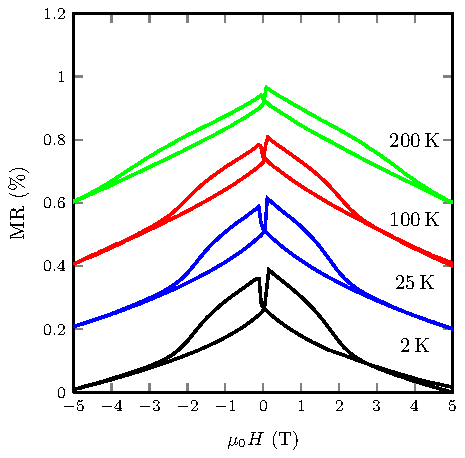
\includegraphics[width=1.0\columnwidth]{Transport-Fig5.pdf}
\caption{MR of a pseudo spin valve \ce{Mn2Ru$_x$Ga}(15)/\ce{Cu}(2.8)/[\ce{Co}(
0.2)/\ce{Pd}(0.6)]$_6$/\ce{Ta}(\SI{3}{\nano\metre})  measured at various 
temperatures. The curves have been offset vertically for clarity.  The inset 
shows the temperature variation of the GMR contribution with a fit to $T^{0.5
}$ dependence.}
\label{fig:gmr}
\end{figure}

%section on GMR
Finally we measured the magnetoresistance (MR) properties of the \ce{MRG}/\ce{
Cu}/[\ce{Co}/\ce{Pd}] samples at different temperatures from \SIrange{2}{300}{
\kelvin}. The MR was measured on unpatterned films in the current-in-plane 
configuration. A MR effect was cleared observed at \SI{2}{\kelvin}, and 
persists even at room temperature as shown in Fig. \ref{fig:gmr}. The 
observed MR is however quite low ($\sim \num{0.15}$) even at \SI{4}{\kelvin} 
which may be due to two effects: Firstly considering the transfer between 
separate deposition chambers for the \ce{MRG} and \ce{Cu}/[\ce{Co}/\ce{Pd}] 
layers, some interfacial contamination or oxidation of the \ce{Mn} can be 
expected.  Secondly, based on the results shown for the thickness dependence 
of the \ce{MRG} films, as discussed above, we find that the films are 
increasingly strained as the thickness of the film is reduced. This causes a 
variation in the spin-dependent transport properties and compensation of the 
two magnetic sub lattices, compared to the thicker films. Furthermore we 
assume that magnetic domains are present in the MRG film as in 
antiferromagnets; GMR is lost relatively quickly due to domain structuring 
and imperfect rotation of the magnetisation in the two electrodes, as 
evidenced by dispersed switching field range as shown in the electronic 
transport (Fig. \ref{fig:she}, and \ref{fig:gmr}).

\section{Conclusion}
\label{sec:conclusion}
We have shown above that the spin-dependent transport properties of \ce{Mn2Ru$%
_x$Ga} are tuneable with both the Ru concentration $x$ and strain. Recent 
\textit{ab inito} calculations \cite{galanakisJAP2013} while providing some 
insight into the electronic structure, does not give convincing arguments 
explaining the variation of the transport properties both with varying Ru 
concentration $x$ and strain. Above we have shown that for a Ru concentration 
$x\approx\num{0.7}$, which shows practically zero magnetization, the sign of 
the spontaneous Hall effect is reversed, indicating the reversal of the 
majority spin channel. Concurrently the spontaneous Hall angle is maximised 
which would imply a reduction in the carrier concentration and high spin 
polarisation that point towards a half metallic state. We also show that by 
varying the tetragonal distortion at a particular Ru composition, we can tune 
the compensation of the two Mn sub lattices to be at a relavant temperature 
regime at above or below room temperature. 
The initial demonstration of magnetoresistance in pseudo-spin-valves with an 
\ce{MRG} electrode indicates that while we are able to observe a MR effect, 
further understanding of the magnetic domain and micromagnetic structures are 
necessary for improving device performance. 
 
\section{Acknowledgements}
\label{sec:acknowledgements}
This work was supported by Science Foundation Ireland through AMBER, and from 
grant 13/ERC/I2561. KR acknowledges financial support from the
European Community's Seventh Framework Programme IFOX, NMP3-LA-2010-246102. 
DB acknowledges financial support from IRCSET. The authors would like to 
thank H. Kurt, M. \v{Z}ic and T. Archer for fruitful discussions.

\bibliography{transp}
\end{document}